% This is where Assessors will be looking for signs of success and for evidence of thorough and systematic 
% evaluation as discussed in Section 8.3. Sample output, tables of timings and photographs of workstation screens,
% oscilloscope traces or circuit boards may be included. A graph that does not indicate confidence intervals will 
% generally leave a professional scientist with a negative impression.

% As with code, voluminous examples of sample output are usually best left to appendices or omitted altogether.
% There are some obvious questions which this chapter will address. How many of the original goals were achieved? 
% Were they proved to have been achieved? Did the program, hardware, or theory really work?
% Assessors are well aware that large programs will very likely include some residual bugs. It should always be 
% possible to demonstrate that a program works in simple cases and it is instructive to demonstrate how close it 
% is to working in a really ambitious case.

% ~2000 words

\documentclass[final,rdr32.tex]{subfiles}
\begin{document}

\chapter{Evaluation}

This chapter describes the results obtained, as well as the evaluation methods and metrics used. Possible optimisations and relevant factors affecting accuracy are also discussed.

\section{LSA64 Results}

\subsection{5-label Training}

The model was tested on the LSA64 dataset, using both the basic \verb|dtw-python| implementation and the \verb|fastdtw| one. The model was trained on a sample of five different labels for sign gestures: Accept, Appear, Argentina, Away, and Barbecue. Accept, Appear, and Barbecue require both hands whereas the Argentina and Away can be performed with a single hand. A set of 50 videos, 10 for each label was used for testing. The accuracy for different amount of training data are as follows:

\begin{table}[!h]
    \begin{center}
        \begin{tabular}{ |c|c|c| }
            \hline
            Num. of videos & Accuracy (dtw-python) & Accuracy (fastdtw) \\
            \hline
            1              & 0.78                  & 0.78               \\
            5              & 0.80                  & 0.72               \\
            10             & 0.94                  & 0.74               \\
            \hline
        \end{tabular}
    \end{center}
    \caption{Results using dtw-python}
    \label{tab:accuracy}
\end{table}

As Table \ref{tab:accuracy} shows, the accuracy of the model increases as the number of training videos per label increases. \verb|dtw-python| obtains better results than \verb|fastdtw| consistently, with only the case of using a single video per label yielding a similar accuracy. This suggests that \verb|fastdtw| is as good as \verb|dtw-python| for cases where there is a low amount of training data. Further evidence is needed to make a conclusion. This will be examined in further sections.

The effect of using a different amount of training data is discussed further, including effects due to the number of hands, and how each implementation responds to different labels.


\subsubsection{Training on 1 video per label}

Using only a single video per label resulted in the following:

\begin{figure}[H]
    \begin{center}
        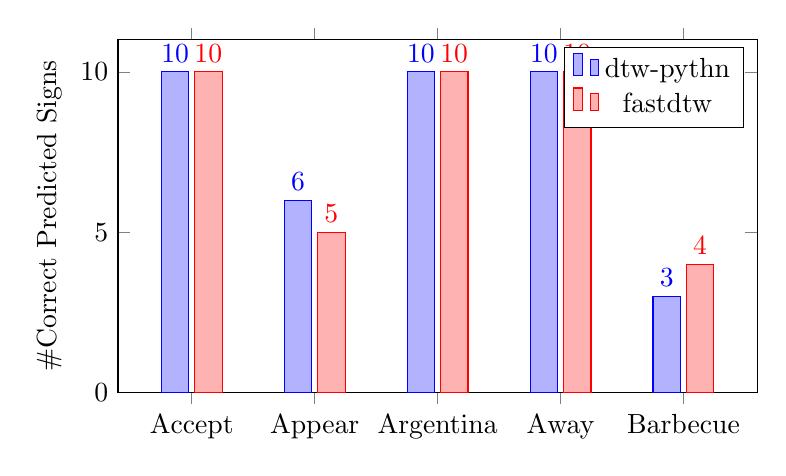
\begin{tikzpicture}
            \pgfplotsset{%
                width=.8\textwidth,
                height=.5\textwidth
            }
            \begin{axis}
                [
                    ybar,
                    enlarge x limits=0.15,
                    ymin=0,
                    ylabel={\#Correct Predicted Signs},
                    symbolic x coords={Accept, Appear, Argentina, Away, Barbecue},
                    xtick=data,
                    nodes near coords,
                    nodes near coords align={vertical},
                ]
                \addplot coordinates {(Accept,10) (Appear,6) (Argentina,10) (Away,10) (Barbecue,3)};
                \addplot coordinates {(Accept,10) (Appear,5) (Argentina,10) (Away,10) (Barbecue,4)};
                \legend{dtw-pythn, fastdtw}
            \end{axis}
        \end{tikzpicture}
    \end{center}
    \caption{Number of correctly predicted signs per label, using one video per label for training}
    \label{bar:one}
\end{figure}

Appear and Barbecue seem to perform poorly on both implementations. They both involve two hands, but Accept does as well and performs very well nevertheless. Other factors that might affect the performance could include:

\begin{itemize}
    \item Appear is executed relatively fast, and part of the hand is hidden during the execution of the sign. This could be affecting with the mediapipe detection.
    \item Barbecue uses both hands in a horizontal position. This seems to make it hard for mediapipe to locate the landmarks for the hands.
\end{itemize}

\newpage


\subsubsection{Training on 5 videos per label}

\begin{figure}[H]
    \begin{center}
        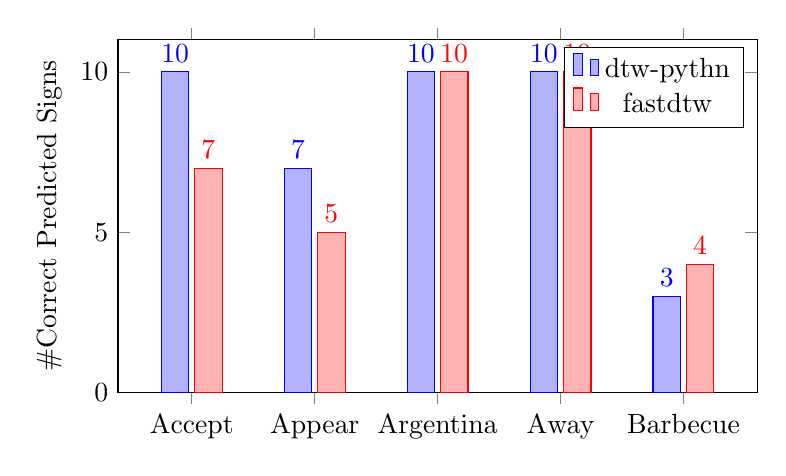
\begin{tikzpicture}
            \pgfplotsset{%
                width=.8\textwidth,
                height=.5\textwidth
            }
            \begin{axis}
                [
                    ybar,
                    enlarge x limits=0.15,
                    ymin=0,
                    ylabel={\#Correct Predicted Signs},
                    symbolic x coords={Accept, Appear, Argentina, Away, Barbecue},
                    xtick=data,
                    nodes near coords,
                    nodes near coords align={vertical},
                ]
                \addplot coordinates {(Accept,10) (Appear,7) (Argentina,10) (Away,10) (Barbecue,3)};
                \addplot coordinates {(Accept,7) (Appear,5) (Argentina,10) (Away,10) (Barbecue,4)};
                \legend{dtw-pythn, fastdtw}
            \end{axis}
        \end{tikzpicture}
    \end{center}
    \caption{Number of correctly predicted signs per label, using 5 videos per label for training}
    \label{bar:two}
\end{figure}

We note the same inconsistencies that are present in Figure \ref{bar:one}. \verb|fastdtw| also performs slightly less efficiently overall compared to \verb|dtw-python|. It is important to note however that \verb|fastdtw| gets all the signs predicted correctly for signs involving a single hand (Argentina and Away). This indicates possibility for optimisation in further implementations.

\newpage

\subsubsection{Training on 10 video per label}

\begin{figure}[H]
    \begin{center}
        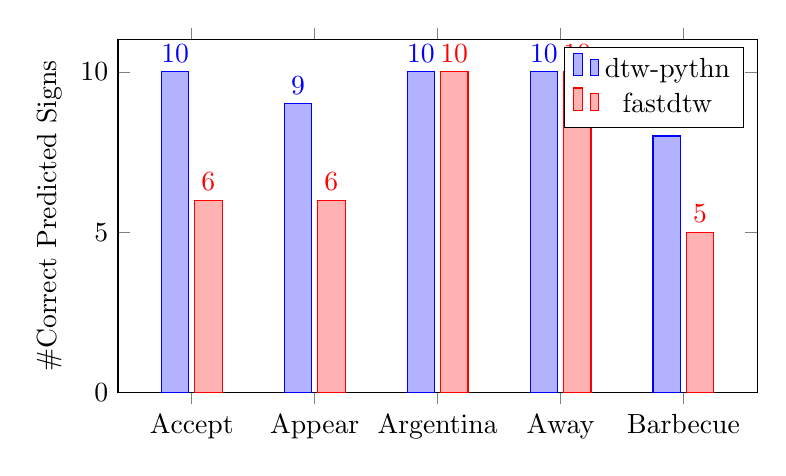
\begin{tikzpicture}
            \pgfplotsset{%
                width=.8\textwidth,
                height=.5\textwidth
            }
            \begin{axis}
                [
                    ybar,
                    enlarge x limits=0.15,
                    ymin=0,
                    ylabel={\#Correct Predicted Signs},
                    symbolic x coords={Accept, Appear, Argentina, Away, Barbecue},
                    xtick=data,
                    nodes near coords,
                    nodes near coords align={vertical},
                ]
                \addplot coordinates {(Accept,10) (Appear,9) (Argentina,10) (Away,10) (Barbecue,8)};
                \addplot coordinates {(Accept,6) (Appear,6) (Argentina,10) (Away,10) (Barbecue,5)};
                \legend{dtw-pythn, fastdtw}
            \end{axis}
        \end{tikzpicture}
    \end{center}
    \caption{Number of correctly predicted signs per label, using 10 videos per label for training}
    \label{bar:three}
\end{figure}

Accuracy is higher overall for this training set. We note the same lower accuracy for \verb|fastdtw| when it comes to two-handed signs and the same bias against Appear and Barbecue.

\subsection{Left-handed Videos Testing}

The model supports left-handed detection as well, even when trained on right-handed videos. Testing was conducted in a similar fashion on the same testing data used for right-handed testing, but with all of the videos flipped instead. The training data consisted of the same videos used for the \textit{five videos per label} criteria.

\section{BSLDict Results}

\section{User Study}

As this project involves real-time detection, a user study was conducted to measure the usability of the model in real-time and to also evaluate its accuracy. The aim of the user study was to establish if the model was suitable to be used for real-time detection and if the \verb|fastdtw| implementation was faster than the \verb|dtw-python| implementation.

\section{Methodology}

A group of 5 participants took turns performing sign language gestures that are trained on. They are provided with a few examples from the testing data to familiarise themselves with the gestures. The user study is carried out separately on the LSA64 dataset and the BSLDict dataset.

The metrics that are measured include the overall accuracy of the model, the accuracy per class, and a confusion matrix. Given that the model is not optimised to detect negatives, it is expected that the model yields poor results when it comes to detecting them. However, it is of interest to know about its performance so that this aspect can be improved in future work.

\section{LSA64 Testing}

\section{BSLDict Testing}



\end{document}